% Chapter Template

\chapter{Literature Review} % Main chapter title

\label{Chapter2} % Change X to a consecutive number; for referencing this chapter elsewhere, use \ref{ChapterX}

\lhead{Chapter 2. \emph{Literature Review}} % Change X to a consecutive number; this is for the header on each page - perhaps a shortened title

%----------------------------------------------------------------------------------------
%\t\tSECTION 1
%---------------------------------------------------------------------------------------
\section{Motion Forecasting}

Motion forecasting has been a long-standing problem in robotics and autonomous driving. Early approaches relied on physics-based models, such as the constant velocity and constant acceleration models. While simple and efficient, these models fail to capture the complex and interactive nature of real-world traffic scenarios.

With the advent of machine learning, classical methods like Kalman filters, Hidden Markov Models (HMMs), and Gaussian Processes were employed to model the uncertainty and dynamics of motion. However, these models often struggle with the high dimensionality and non-linearity of multi-agent systems.

In recent years, deep learning has become the dominant paradigm for motion forecasting \citep{Shi2025MotionFF}. Recurrent Neural Networks (RNNs), particularly Long Short-Term Memory (LSTM) networks, have been widely used to model the sequential nature of trajectory data. Convolutional Neural Networks (CNNs) have also been used to extract features from rasterized scene images. More recently, attention mechanisms have been introduced to better capture the complex dependencies in motion data \citep{Mao2021Multi-levelMA, Ding2022DeepLW}.

\section{Agent-Centric vs. Scene-Centric Approaches}

Modern deep learning-based motion forecasting models can be broadly categorized into two paradigms: agent-centric and scene-centric.

\textbf{Agent-centric} approaches model the trajectory of each agent independently, often using RNNs to encode the past motion and decode the future. These models are computationally efficient but often fail to capture the complex interactions between agents.

\textbf{Scene-centric} approaches, on the other hand, process all agents in a scene simultaneously, often using a shared architecture like a CNN or a graph neural network. These models are better at capturing interactions but can be computationally expensive and may struggle with a large number of agents.

\section{AgentFormer}

AgentFormer \citep{yuan2021agentformer} is a transformer-based architecture designed for multi-agent trajectory forecasting. It addresses the limitations of previous methods that model the temporal (time) and social (agent interactions) dimensions of trajectories separately. The key innovation of AgentFormer is its ability to model these two dimensions simultaneously, allowing for a more holistic understanding of the scene dynamics.

\subsection{Simultaneous Socio-Temporal Modeling}

Unlike traditional approaches that first encode temporal information for each agent and then model social interactions (or vice-versa), AgentFormer processes a flattened sequence of all agents' trajectories across all timesteps. This allows the model to learn direct relationships between an agent's state at one time and another agent's state at a future time.

\subsection{Agent-Aware Attention}

A core contribution of AgentFormer is the novel \textbf{agent-aware attention} mechanism. Standard attention mechanisms in transformers do not distinguish between different agents in a sequence. To overcome this, AgentFormer uses two sets of queries and keys: one for \textbf{intra-agent attention} (an agent attending to its own past states) and another for \textbf{inter-agent attention} (an agent attending to the states of other agents). This is achieved through a masking mechanism that identifies whether a query and a key belong to the same agent. This allows the model to learn different patterns for an agent's own motion and its interaction with others.

\subsection{CVAE-based Probabilistic Forecasting}

To model the inherent uncertainty and multi-modality of future trajectories, AgentFormer is built upon a Conditional Variational Autoencoder (CVAE) framework. It introduces a latent variable for each agent to represent its "intent." The model learns a joint distribution over the latent intents of all agents, enabling it to generate socially-aware and diverse future trajectories. The CVAE framework consists of:

\begin{itemize}
    \item \textbf{Past Encoder:} An AgentFormer encoder that processes the past trajectories of all agents to produce a context representation.
    \item \textbf{Future Encoder:} An AgentFormer decoder that processes the ground truth future trajectories (during training) to infer the posterior distribution of the latent variables.
    \item \textbf{Future Decoder:} An autoregressive AgentFormer decoder that takes the context representation and a sampled latent code to generate the future trajectory one step at a time.
\end{itemize}

\begin{figure}[h]
\centering
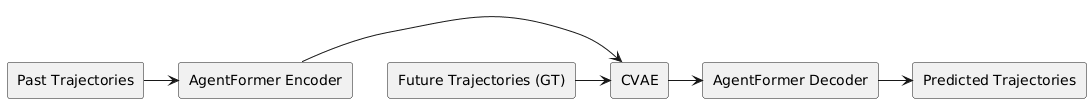
\includegraphics[width=\textwidth]{agentformer_architecture.png}
\caption{Overview of the AgentFormer-based multi-agent trajectory prediction framework. Figure from \citep{yuan2021agentformer}.}
\label{fig:agentformer_architecture}
\end{figure}


\section{Bird's-Eye-View (BEV) Representations}

Bird's-Eye-View (BEV) is a popular representation for scene understanding in autonomous driving. It provides a top-down view of the 3D world, which is a natural and intuitive representation for tasks like object detection, segmentation, and motion planning.

BEV representations have several advantages over other representations, such as camera-view or point cloud representations:

\begin{itemize}
    \item They provide a unified representation of the scene, where objects are represented at their correct metric scale and location.
    \item They are invariant to camera perspective changes.
    \item They are well-suited for downstream tasks like planning and control.
\end{itemize}

\section{BEVDepth}

BEVDepth \citep{li2022bevdepth} is a leading model for generating dense BEV feature maps from multiple camera images. It addresses the challenge of accurately projecting image features into the 3D world by explicitly predicting the depth of each pixel in the image.

The BEVDepth model consists of several key components:

\begin{itemize}
    \item A camera-view encoder that extracts features from each camera image.
    \item A depth prediction network that estimates the depth of each pixel.
    \item A view transformer that lifts the 2D image features into a 3D point cloud using the predicted depth.
    \item A voxel pooling layer that aggregates the 3D points into a dense BEV feature map.
\end{itemize}

BEVDepth has achieved state-of-the-art performance on several BEV segmentation and detection benchmarks. Its ability to generate high-quality BEV features makes it an attractive candidate for providing visual context to motion forecasting models.

\section{Gap in the Literature}

While both AgentFormer and BEVDepth are powerful models in their respective domains, their integration has not been thoroughly explored. AgentFormer excels at modeling agent interactions but lacks a deep understanding of the visual scene. BEVDepth, on the other hand, provides a rich representation of the visual scene but does not directly perform motion forecasting.

This thesis aims to fill this gap by investigating the integration of BEVDepth with AgentFormer. The goal is to leverage the strengths of both models to create a more robust and accurate motion forecasting system. The surprising negative results of this integration, as will be discussed in the following chapters, highlight the challenges of multi-modal fusion and provide valuable insights for future research in this area.

